% 
\titlehead{%
}
%
\subject{\SubjectStyle{%
ANL-OpenCL}}
%
\title{%
Documentation}
%
\subtitle{%
}
%
\author{\AuthorStyle{%
Erwin Müller}}
%
\date{\DateStyle{%
\today}}
%
\publishers{\PublishersStyle{%
\url{https://anl-opencl.anrisoftware.com/}}}
%
\renewcommand{\TheHeadingLogo}{%

\includegraphics[height=1em]{logo.png}}
%
\renewcommand{\TheHeadingAuthor}{%
}
%
%\thanks{footnote }
%
%\lowertitleback{}
%
\uppertitleback{%
}
%
\dedication{\DedicationStyle{%
}}
%
\newcommand{\TheAbstract}{
\begin{center}
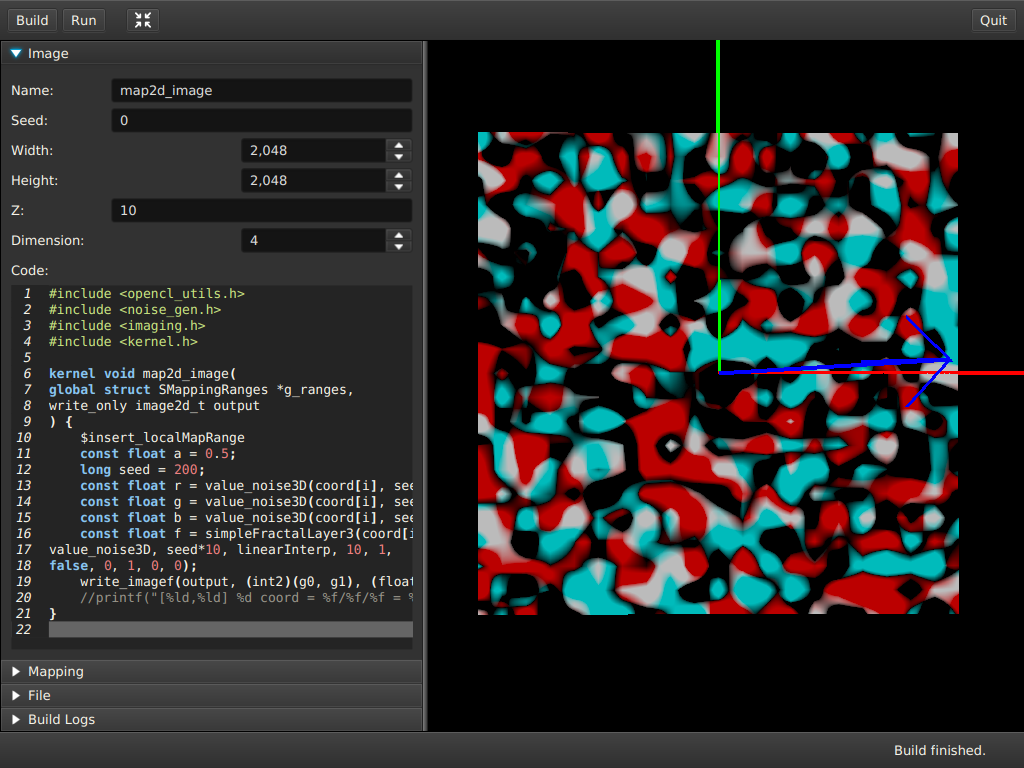
\includegraphics[width=0.8\textwidth]{Screenshot_20211121_152848.png}
\end{center}
The purpose of this document is to describe the \ANLOpenCL/ library, how to
use it to create noise images and how to use the bundled app.
} 
%
